\documentclass[tikz]{standalone} 

    \begin{document} 
     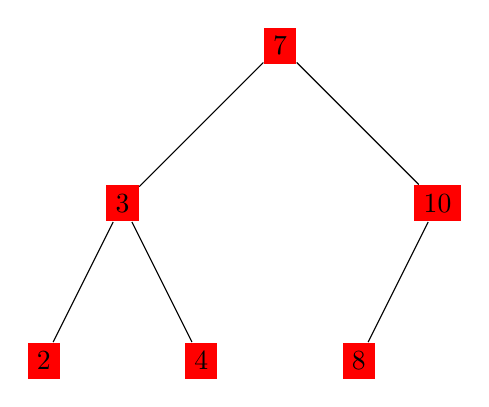
\begin{tikzpicture}[every node/.style={fill=red}, every edge/.style={draw,}] 

       % Hier stehen die Zeichen-Befehle. 
         \coordinate (x7) at (0, 0);
  \coordinate (x3) at (-2, -2);
  \coordinate (x10) at (2, -2);
  \coordinate (x2) at (-3, -4);
  \coordinate (x4) at (-1, -4);
  \coordinate (x8) at (1, -4); 
  \node (n7) at (x7) {$7$};
  \node (n3) at (x3) {$3$};
  \node (n10) at (x10) {$10$};
  \node (n2) at (x2) {$2$};
  \node (n4) at (x4) {$4$};
  \node (n8) at (x8) {$8$}; 
  \draw (n7) edge (n3);
  \draw (n7) edge (n10);
  \draw (n3) edge (n2);
  \draw (n3) edge (n4);
  \draw (n10) edge (n8); 

        \end{tikzpicture} 
        \end{document}